% !TEX root = main.tex
\subsection{第2週:液体金属を用いたpn接合ダイオードの作製}

\subsubsection*{目的}

本実験では,真空装置や成膜装置を使用せずに,液体金属を用いて簡易的なpn接合ダイオードを作製する.  
一般にpn接合ダイオードは,真空中での蒸着やスパッタリングにより電極を成膜するが,これらの方法は装置が高価で,作製に多くの時間を要する.

本手法では,液体金属をSi基板上に直接塗布することで,電極形成を簡便かつ短時間で行い,
実験的に動作するダイオード構造を構築する.


\subsubsection*{作製手順}

\paragraph{⓪ Siウェハーの切り出し}

作製に使用するSiウェハーは,$1.5~\mathrm{cm} \times 1.5~\mathrm{cm}$ のサイズに切り出す.  
切断には \textbf{ファインクリスタルカッター} を用い,以下のようにして行った.

\begin{itemize}
    \item ピカピカの鏡面(n型面)を下にしてろ紙の上に置く
    \item ファインクリスタルカッターで表面に傷をつける
    \item 上下を硝子盤で挟み,指で均等に押して割断する
\end{itemize}

使用した器具はすべて,\textbf{イソプロピルアルコール(IPA)}と\textbf{キムワイプ}で清浄化し,次のものを用いた.


\begin{itemize}
    \item ピンセット(非金属)
    \item ガラス盤
    \item 薬剤紙,ろ紙
\end{itemize}

\begin{figure}[H]
    \centering
    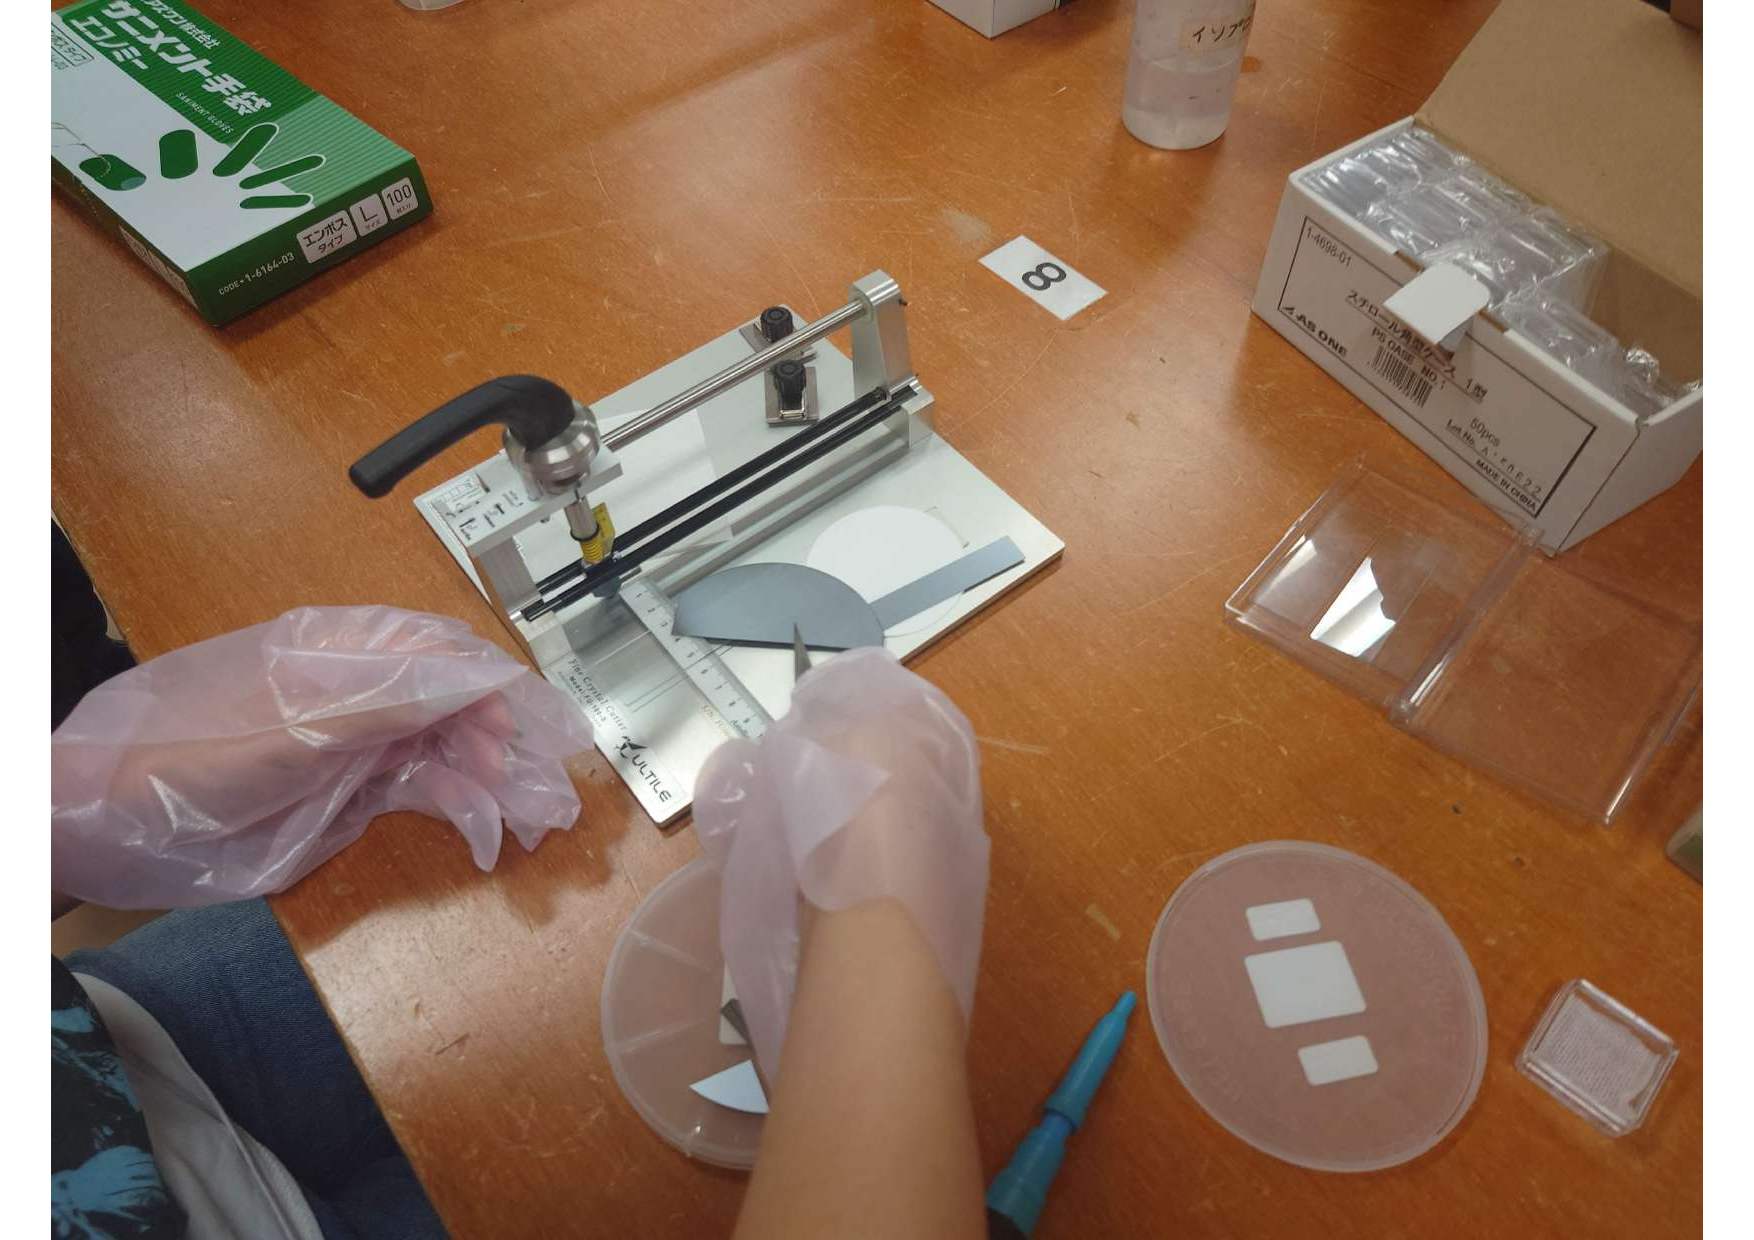
\includegraphics[width=0.6\textwidth]{figure/20250722_131053.pdf}
    \caption{基板切断の様子}
    \label{fig:washing_flow}
\end{figure}

\begin{figure}[H]
    \centering
    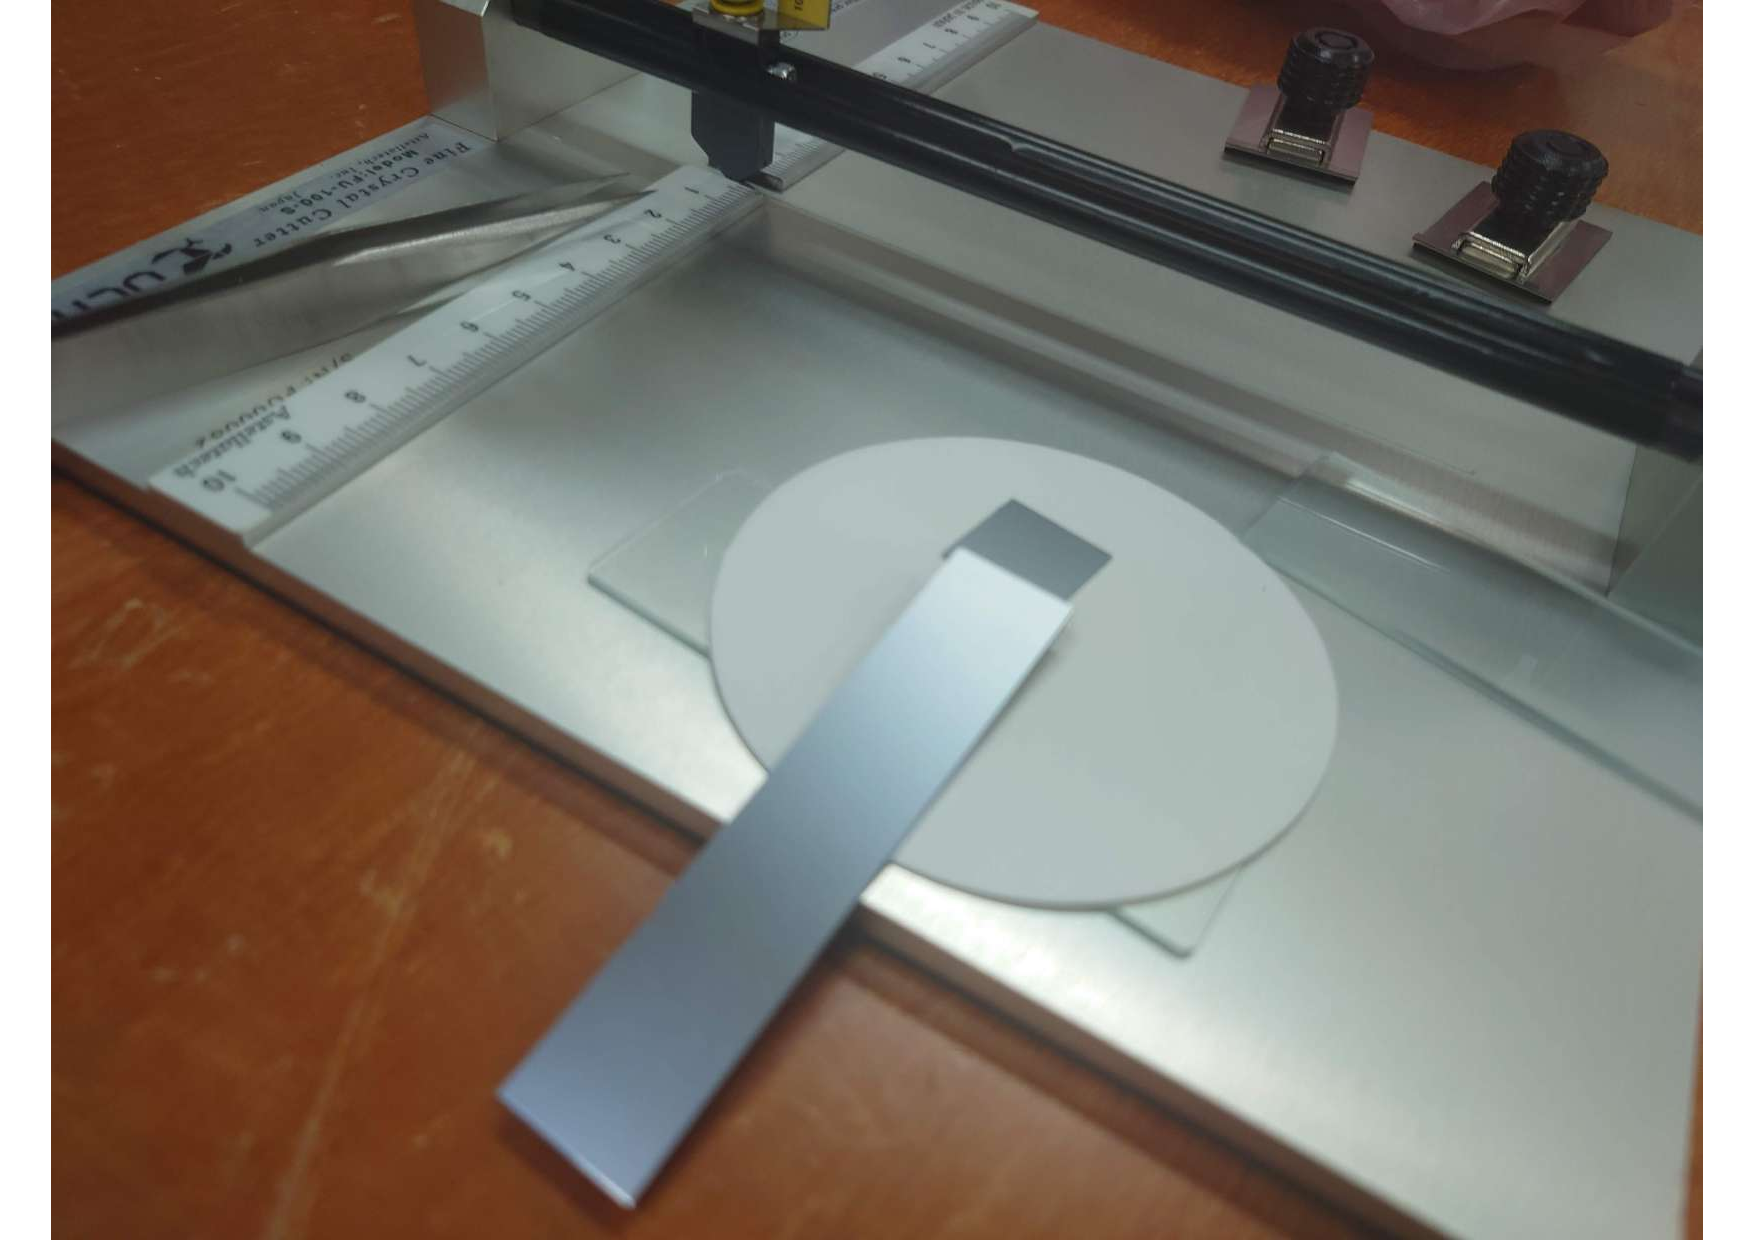
\includegraphics[width=0.6\textwidth]{figure/20250722_132215.pdf}
    \caption{基板切断}
\end{figure}


\paragraph{① 基板の洗浄}

基板の洗浄は,接合界面の品質を確保するために極めて重要である.  
微粒子,金属汚染,有機汚染,イオン汚染,自然酸化膜などを除去するため,以下の工程で行った.


\begin{table}[H]
    \centering
    \caption{基板洗浄プロセス}
    \label{tab:wash_process}
    \begin{tabular}{cl}
        \hline
        工程 & 内容 \\
        \hline
        (1) & Si基板を台にセット \\
        (2) & アセトンによる5分間の超音波洗浄 \\
        (3) & IPAによる5分間の超音波洗浄 \\
        (4) & 純水で5分間オーバーフロー洗浄 \\
        (5) & 希フッ酸洗浄(酸化膜除去) \\
        (6) & 純水で5分間オーバーフロー洗浄 \\
        (7) & フローにより乾燥 \\
        \hline
    \end{tabular}
\end{table}

\begin{figure}[H]
    \centering
    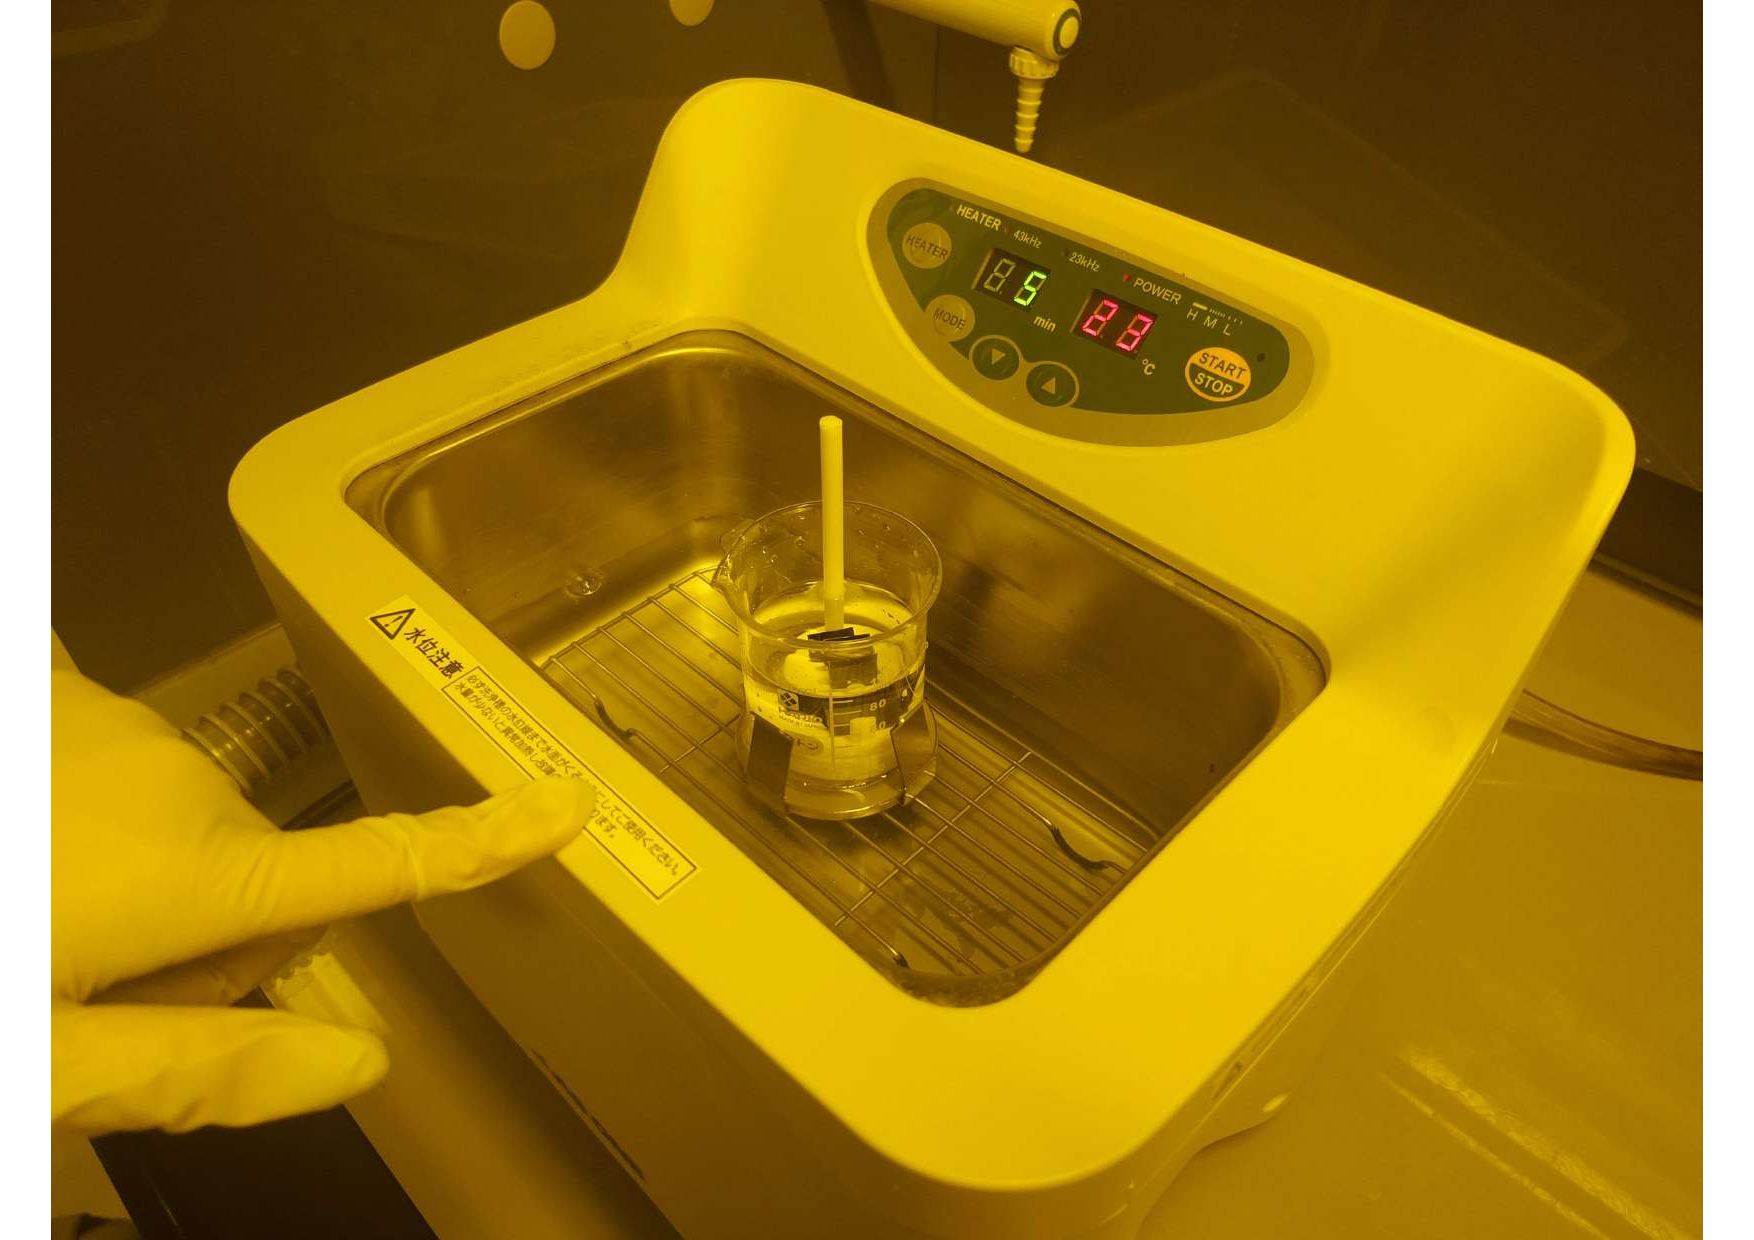
\includegraphics[width=0.6\textwidth]{figure/20250722_141148.pdf}
    \caption{基板洗浄の様子}
    \label{fig:washing_flow}
\end{figure}

※ 希フッ酸は腐食性が高いため,ポリエチレン製の手袋とピンセットを使用して安全に作業を行った.酸化膜除去の目安は「基板表面が水をはじく状態」である.


\paragraph{② 液体金属による電極形成}

洗浄後のSi基板に対して,以下の工程で電極を形成した(図\ref{fig:electrode_process} 参照).

\begin{enumerate}
    \item Si基板表面に金属マスクを設置
    \item マスクの上に液体金属を滴下し,ヘラで塗布
    \item 金属マスクをゆっくり剥がす
    \item 銅板にも液体金属を塗布
    \item シリコン基板裏面を銅板と接着
    \item ダイオード構造が完成
\end{enumerate}

\begin{figure}[H]
    \centering
    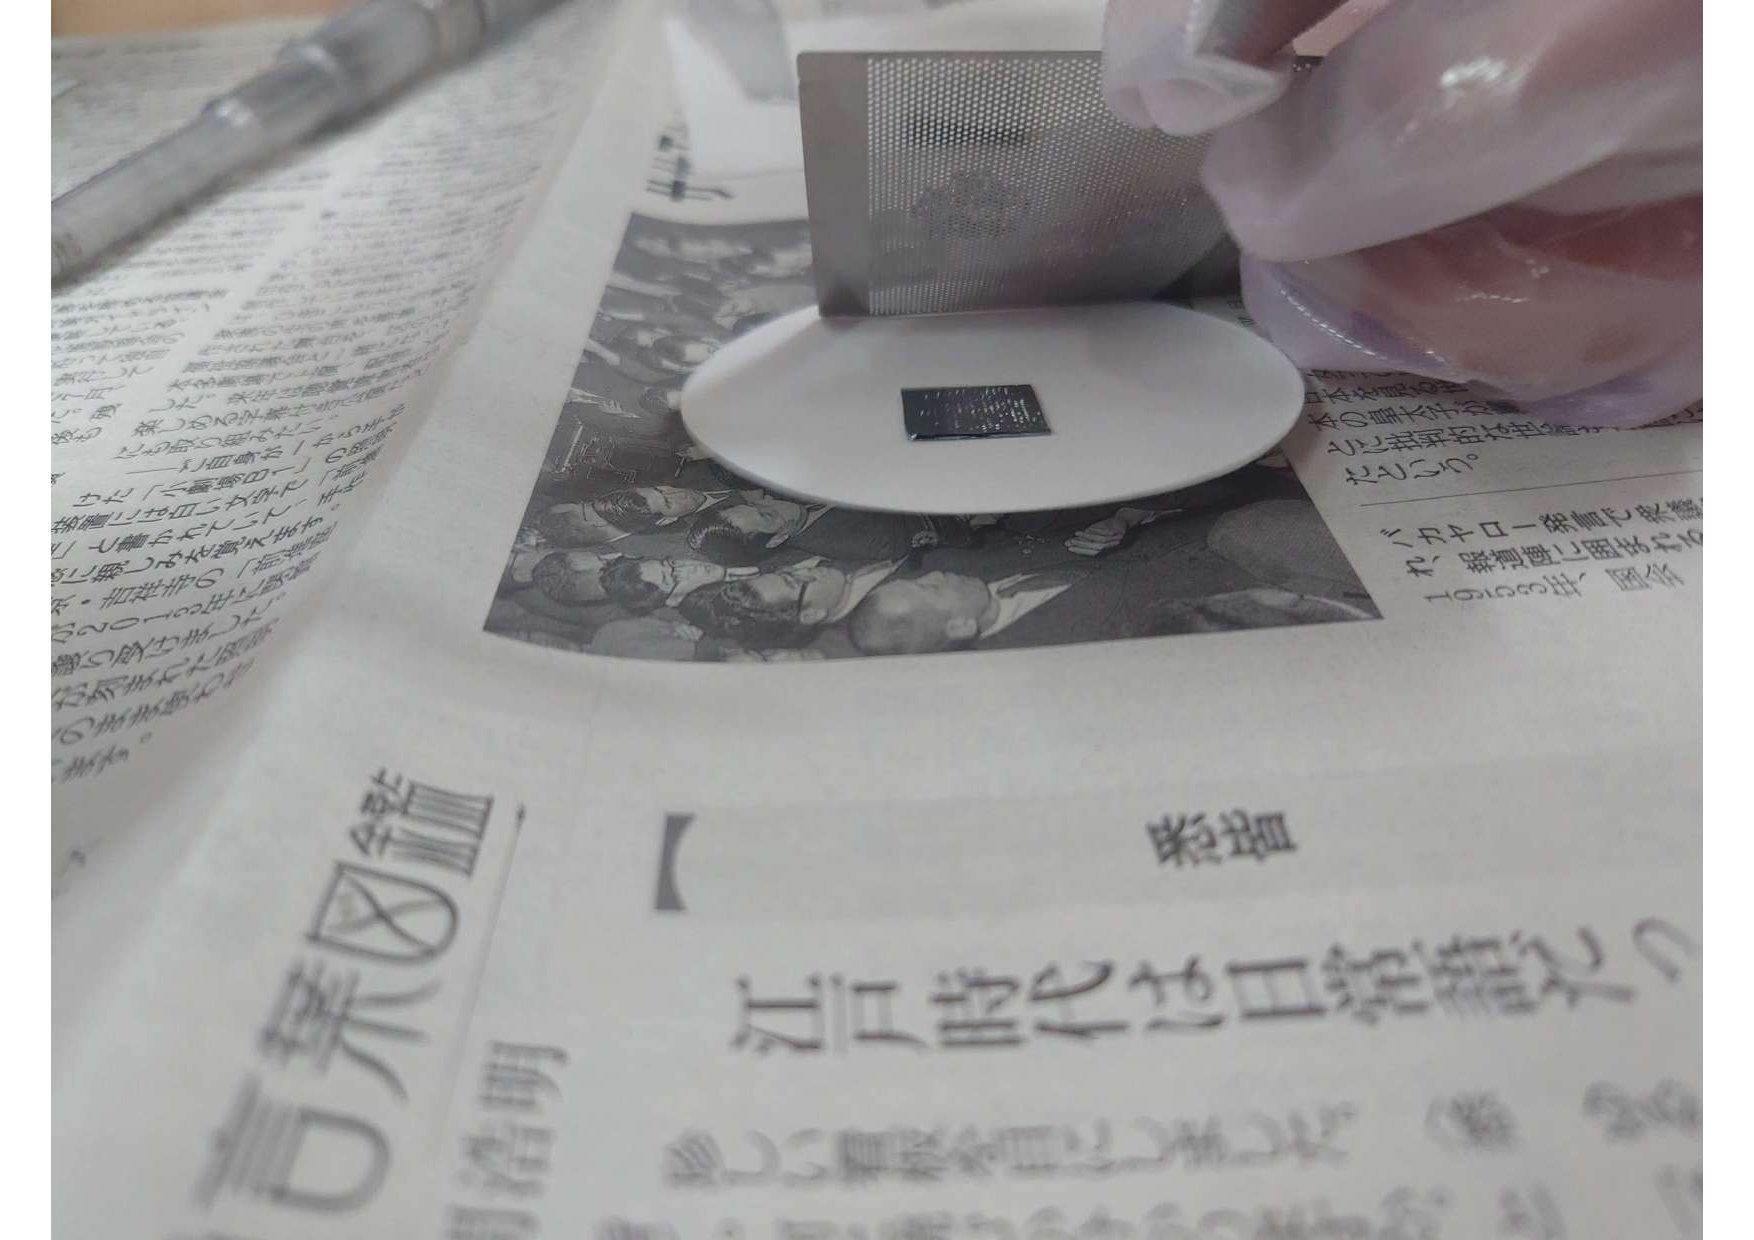
\includegraphics[width=0.6\textwidth]{figure/20250722_155957.pdf}
    \caption{液体金属による電極形成}
    \label{fig:electrode_process}
\end{figure}

\begin{figure}[H]
    \centering
    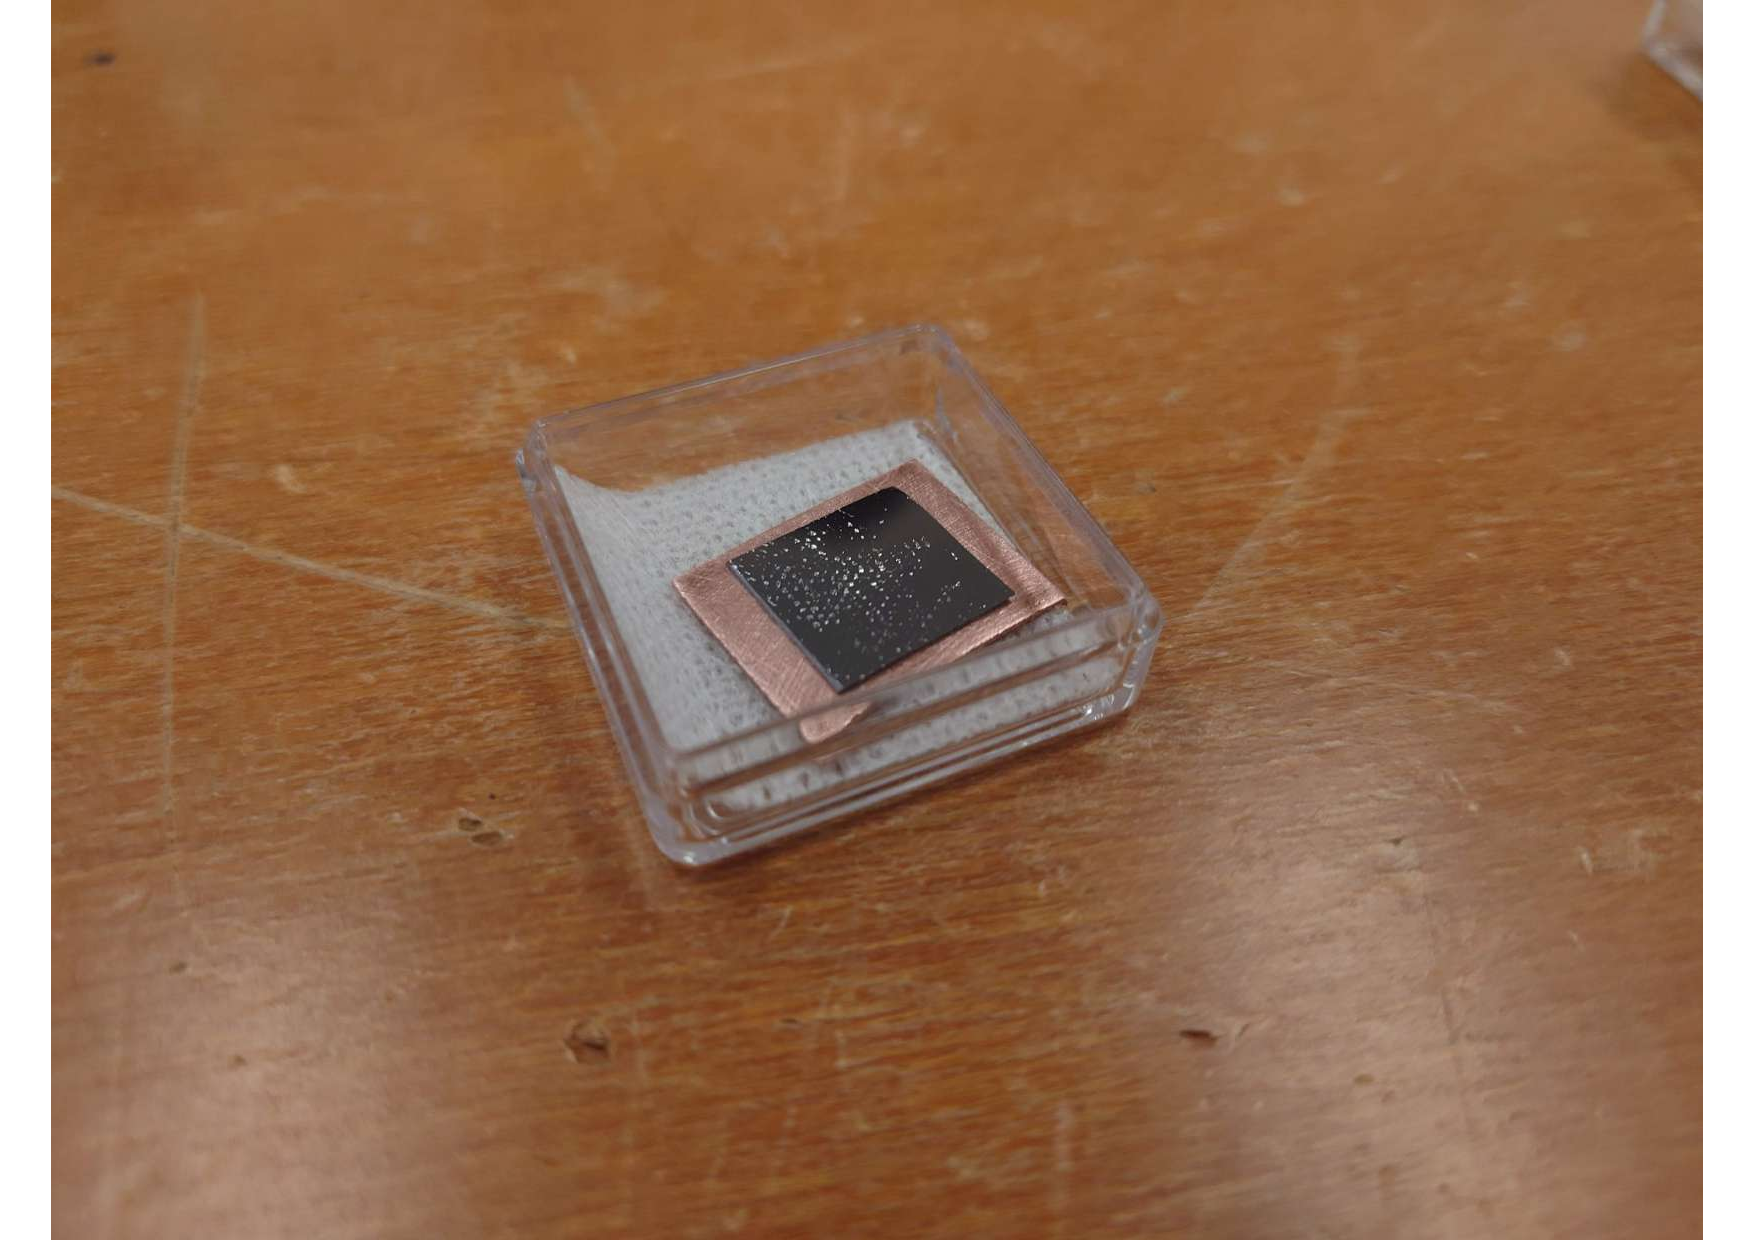
\includegraphics[width=0.6\textwidth]{figure/20250722_160238.pdf}
    \caption{完成物の外観}
\end{figure}


\paragraph{注意点}

\begin{itemize}
    \item 銅板は使用前に表面を紙やすりなどで研磨し,酸化膜を除去する.
    \item Si基板の「表面」(鏡面)と「裏面」(ザラザラ面)を間違えないこと.
    \item 銅板との接着時に圧をかけすぎると,液体金属が側面から溢れ,短絡する危険がある.はみ出した部分は吸い取っておく.
\end{itemize}

\begin{figure}[H]
    \centering
    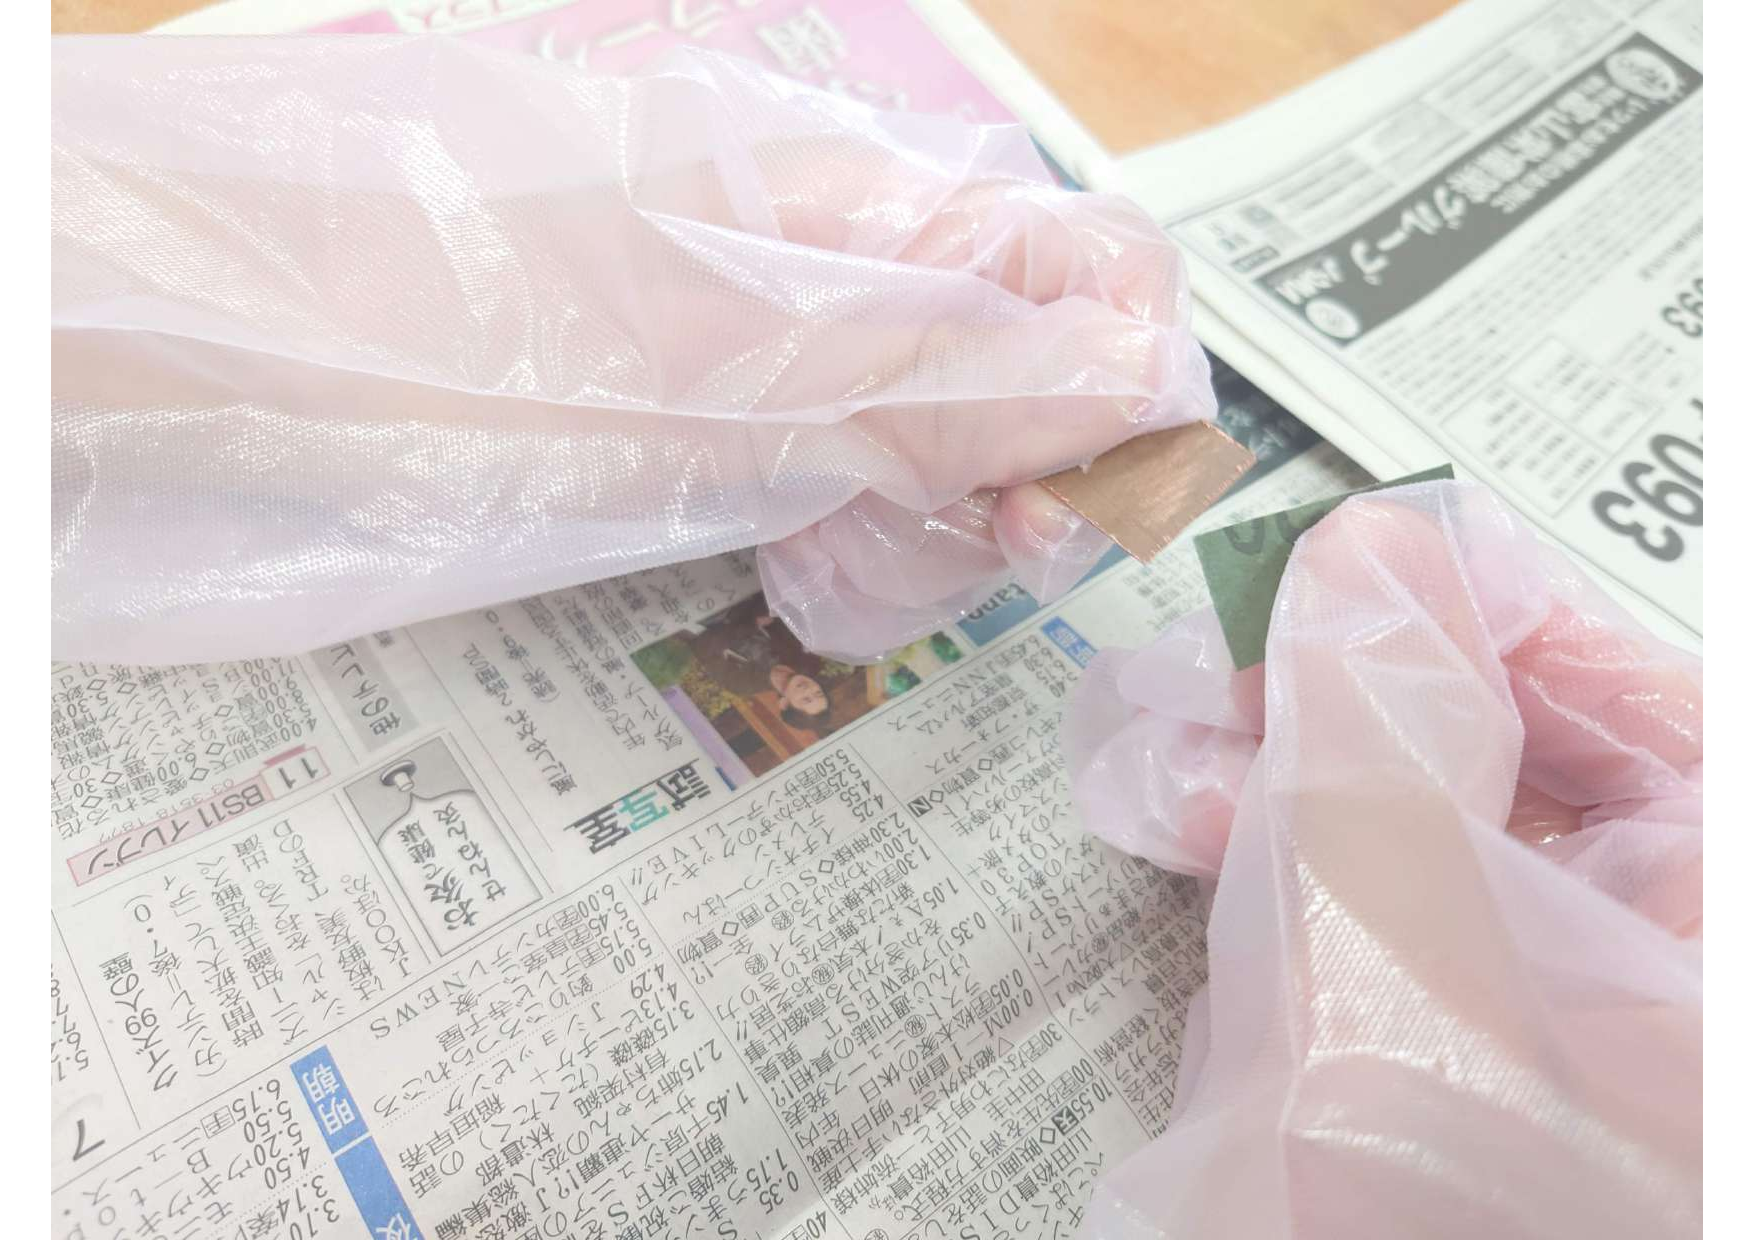
\includegraphics[width=0.6\textwidth]{figure/20250722_153608.pdf}
    \caption{銅板を紙やすりで研磨}
\end{figure}